\chapter{Bayesian Inference}
\label{chap:bay}
%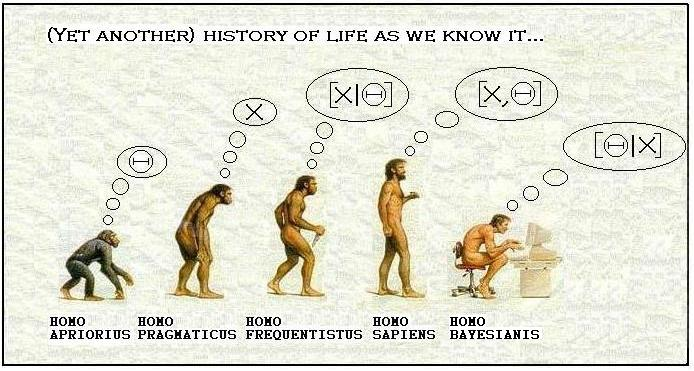
\includegraphics[width=\textwidth]{bayesian_evol}

\epigraph{We anticipate the sun will rise tomorrow, not just because it has always done so far, but because this is predicted by {\em models}, which accord with {\em data}. Any perceived failure of the sun to rise would more likely be a hallucination.}{\davidmackay{}}

\begin{itemize}
  \item BRIEF intro to difference between bayesian and frequentist, and the nature of probability
    \begin{itemize}
      \item Continuous vs. Discrete
      \item Aleatoric vs. Epistemological \davidspiegelhalter
    \end{itemize}
  \item Parameter estimation and model comparison
    \begin{itemize}
      \item Example? (e.g.\ coin flipping, --- anything better?)
    \end{itemize}
  \item Sampling as method for describing high-dimensional probability distributions.
    \begin{itemize}
      \item MH as good technique
      \item Need for evidences
    \end{itemize}
\end{itemize}


Science is not the search for truth. Instead, scientists concern themselves with the construction of models. These models have their relative merit determined using data.\footnote{The opening statement of this chapter was in fact the first thing \rafiblumenfeld{} said to us for our part IB Physics supervisions.}

% Mathematics -- if then, conditional truth
% Science -- weaker: observations -> possibilities 

\newcommand{\Probc}[2]{\mathrm{P}\left(#1\middle|#2\right)}
\newcommand{\Prob}[1]{\mathrm{P}\left(#1\right)}

\section{Probability}
\label{sec:bay:prob}

Probability is the mathematical language of uncertainty. It is a methodology of assigning a numerical weighting to outcomes or {\em events}. An event is any subset of the sample space $\Omega$. Some examples of discrete and continuous sample spaces are:
\begin{enumerate}
  \item The outcome of a coin flip $\Omega_1=\{\mathrm{Heads},\mathrm{Tails}\}$.
  \item The measured position of an electron $\Omega_2=\mathbb{R}$.
\end{enumerate}
For example, an event could be that the electrons position $x$ is measured to be $-1<x<0.5$. The role of probability is to assign a weighting to all subsets, which roughly corresponds to the ``chance'' that such an event would occur. Probability should therefore be additive:
\begin{equation}
  A,B \mathrm{\ disjoint} \Rightarrow \Prob{A \cup B} = \Prob{A} + \Prob{B}.
  \label{eqn:bay:add}
\end{equation}
One also normalises the probability distribution so that $\Prob{\Omega} = 1$. The above is effectively a paraphrasing of Kolmogorov's axioms of probability.

In addition, if one has two disjoint sample spaces, for example $\Omega_1$ and $\Omega_2$ mentioned above, one may combine these into a single samples space ${\Omega=\Omega_1\otimes\Omega_2}$, then probability should be multiplicative.





This entire section may be summarised succinctly and formally as:
\begin{quote}
  Probability is any additive mapping $\mathrm{P}$ from the power set $2^\Omega$ of the sample space $\Omega$ to $[0,1]\in \mathbb{R}$, such that $\Prob{\Omega}=1$.
\end{quote}
\johnskilling{} has derived probability from measurement-theoretical grounds\citep[chap. 1]{Bayesian_methods_in_cosmology}, which provides a more intuitive backing to the definition.

\begin{figure}
  \centerline{%
    \def\firstcircle{(-0.75,0) circle (1.5)}
\def\secondcircle{(0.75,0) circle (1.5)}

\begin{tikzpicture}
  \draw \firstcircle;
  \draw \secondcircle;
  \draw (-3,-2) rectangle (3,2);

  \begin{scope}
    \fill[blue!30!white] \firstcircle;
    \clip \secondcircle;
  \end{scope}

  \begin{scope}
    \clip \firstcircle;
    \fill[blue!60!white] \secondcircle;
  \end{scope}

  \draw[above left] node at (-1,0) {\(A\)};
  \draw[above right] node at (1,0) {\(B\)};
  \draw[below ] node at (0,0) {\(A\cap B\)};
  \draw[below left] node at (3,2) {\(\Omega\)};


\end{tikzpicture}


  }
  \caption{Beer-mat mathematics. This diagram is how \edjaynes{} explained Bayes' theorem to a young \stevegull{}. Out of the entire sample space $\Omega$, if we observe $A$ to be true (blue region), then the probability of $B$ given that we know $A$ is simply $\Prob{A\cap B}/\Prob{A}$. Bayes' theorem then follows by rearrangement and symmetry.}
\end{figure}


From this definition, it is useful to define conditional probability via:
\begin{equation}
  \Probc{B}{A} = \frac{\Prob{A\cap B}}{\Prob{A}}.
  \label{eqn:bay:cond}
\end{equation}
Multiplying both sides by $\Prob{A}$, and noting the symmetrical alternative:
\begin{equation}
  \Probc{B}{A}\Prob{A} = \Prob{A\cap B} = \Probc{A}{B}\Prob{B},
  \label{eqn:bay:sym}
\end{equation}
one may then derive Bayes' theorem:
\begin{align}
  \Probc{B}{A} &= \frac{\Probc{A}{B}\Prob{B}}{\Prob{A}}.\\
  \label{eqn:bay:bayes}
  \tag{Bayes' Theorem}
\end{align}


\section{Bayesian vs.\ Frequentist}
\label{sec:bay:bayesian_frequentist}

Whilst the previous section outlined the properties that probability must satisfy, it has not detailed how one should assign probability. Indeed, we have merely referred to probability as a measure of ``chance'', but declined to define what this means.

The Frequentist school of thought defines probability as:
\begin{description}
  \item[Frequentist Probability:]``The limiting relative frequency of an event.''
\end{description}
I.e.\ if a coin has $\Prob{\mathrm{Head}}=\frac{1}{2}$, then if you were to toss it an arbitrarily large number of times, the fraction of times one would get closer and closer to $\frac{1}{2}$. There is certainly nothing incorrect about this definition, but it is too stringent. Most people's experiences with probability will likely involve betting scenarios. If a sports team's victory has betting odds of $5:1$ (or $\Prob{\mathrm{Win}} = \frac{1}{6}$), one {\em cannot\/} repeat the experiment an arbitrarily large number of times. The alternative definition of probability is {\em Bayesian\/}:
\begin{description}
  \item[Bayesian Probability:] ``A degree of belief that an event will occur.'' 
\end{description}
Note that Bayesian probability is {\em subjective}, it matters who's degree of belief one is considering. Probabilities are assigned only with a given state of knowledge. 

Pure mathematics deals in relative truth or falsity, i.e.\ given initial assumptions, all statements are assigned to the set $\{F,T\}\equiv\{0,1\}$. Bayesian probability can be thought of as a blurring of this process, namely from initial assumptions, various conclusions are assigned a number between $[0,1]$.

\section{Parameter Estimation \& Model Comparison}
\label{sec:bay:model_comp}


\section{Sampling}
\label{sec:bay:samp}

